%----------------------------------------------------------------------------------------
% БҮЛЭГ 5: ТУРШИЛТ СУДАЛГАА БА ҮР ДҮН
%----------------------------------------------------------------------------------------

\chapter{Туршилт судалгаа ба үр дүн}

\section{Туршилтын орчин}

Туршилтыг дараах техник хангамжийн нөхцөлд явуулна:

\begin{table}[htbp]
\centering
\caption{Туршилтын орчны тохиргоо}
\label{tab:experiment_env}
\begin{tabular}{ll}
\hline
\textbf{Бүрдэлхүүн} & \textbf{Тодорхойлолт} \\
\hline
GPU                    & NVIDIA A100 80GB (локал сервер) \\
CPU                    & Intel Xeon 32 core \\
RAM                    & 128 GB \\
Хадгалах санах ой      & 2 TB SSD \\
Python                 & 3.10, PyTorch 2.7.1+cu118 \\
Transformers           & 5.3.0 \\
Нарийвчилсан тохируулга framework  & TRL + PEFT + BitsAndBytes \\
Тасралтгүй хяналт      & WandB + Rich terminal хяналтын самбар \\
Random seed            & 42 (reproducibility-г хангах) \\
\hline
\end{tabular}
\end{table}

\section{Туршилтын өгөгдлийн хуваалт}

\begin{table}[htbp]
\centering
\caption{Өгөгдлийн хуваалт}
\label{tab:data_split_exp}
\begin{tabular}{lcccc}
\hline
\textbf{Хуваалт} & \textbf{Нийт} & \textbf{Хүчирхийлэл} & \textbf{Хүчирхийлэлгүй} & \textbf{Хувь} \\
\hline
Сургалт (Train)          & 1,560 & 801 (51.3\%)       & 759 (48.7\%)       & 80\% \\
Баталгаажуулалт (Val)    & 195   & 105 (53.8\%)       & 90 (46.2\%)        & 10\% \\
Тест (Test)              & 196   & 94 (48.0\%)        & 102 (52.0\%)       & 10\% \\
\hline
\textbf{Нийт}             & \textbf{1,951} & \textbf{1,000 (51.3\%)} & \textbf{951 (48.7\%)} & \textbf{100\%} \\
\hline
\end{tabular}
\end{table}

\section{Үнэлгээний хэмжүүр}

Загварын гүйцэтгэлийг дараах хэмжүүрүүдээр үнэлнэ:

\begin{itemize}
    \item \textbf{Accuracy (нарийвчлал):} Нийт зөв ангилалтын хувь.
    \item \textbf{Precision:} Зодоон гэж ангилсны дотор үнэхээр зодоон байсан хувь.
    \item \textbf{Recall:} Бодит зодооны клипүүдээс зөв илрүүлсэн хувь.
    \item \textbf{F1-Score:} Precision ба Recall-ийн тэнцвэрт дундаж.
    \item \textbf{Токений нарийвчлал:} Нарийвчилсан тохируулгын явцын токен түвшний нарийвчлал.
\end{itemize}

\section{Суурь загвар тогтоолт}

Гарын авлагын Ш-1 шаардлагын дагуу суурь үзүүлэлтийг тогтоосон. Суурь загвар болгон нарийвчилсан тохируулга хийгдээгүй Qwen2.5-VL-7B загварыг ашигласан.

\begin{table}[htbp]
\centering
\caption{Суурь загварын үзүүлэлт}
\label{tab:baseline}
\begin{tabular}{lll}
\hline
\textbf{Метрик} & \textbf{Суурь утга} & \textbf{Зорилтот утга} \\
\hline
Accuracy              & 0.5440                   & $\geq$ 0.9000 \\
F1-score              & 0.6860                   & $\geq$ 0.9000 \\
Recall                & 0.9240                   & $\geq$ 0.9000 \\
GPU VRAM              & 14 GB                     & $\leq$ 16 GB \\
Параметрын тоо        & 7B                        & 7B (хэвээр) \\
\hline
\multicolumn{3}{l}{\footnotesize Суурь утга нь Qwen2.5-VL-7B BASE загварын Val загварын үнэлгээний үр дүн.}
\end{tabular}
\end{table}

\section{Загваруудын харьцуулалт}

Дэвшүүлсэн системийн гүйцэтгэлийг Qwen загварын хувилбаруудтай харьцуулан үнэлэв:

\begin{table}[htbp]
\centering
\caption{Загваруудын хоёртын ангиллын загварын үнэлгээний харьцуулалт}
\label{tab:model_comparison}
{\small
\begin{tabular}{lccc}
\hline
\multirow{2}{*}{\textbf{Загвар}} & \multicolumn{3}{c}{\textbf{Үнэлгээний оноо}} \\
\cline{2-4}
& \textbf{Accuracy} & \textbf{F1} & \textbf{Recall} \\
\hline
Qwen2-VL-7B (2024) & 0.5590 & 0.5980 & 0.6100 \\
Qwen2.5-VL-7B BASE (2025) & 0.5440 & 0.6860 & 0.9240 \\
Qwen3-VL-30B-A3B (2025) & 0.8870 & 0.8950 & 0.8950 \\
\textbf{Qwen2.5-VL-7B fine-tuned} & \textbf{0.9179} & \textbf{0.9238} & \textbf{0.9238} \\
\hline
\end{tabular}
}
\end{table}

\subsection{Загваруудын гаралтын харьцуулалт}

Qwen2-VL-7B, Qwen2.5-VL-7B BASE, Qwen3-VL-30B-A3B болон stillmeta/fight-video-qlora1 загваруудын загварын үнэлгээний гаралтыг
Зураг~\ref{fig:model_comparison}-т харьцуулан үзүүлэв.

\begin{figure}[H]
    \centering
    \begin{subfigure}[t]{0.48\textwidth}
        \centering
        \includegraphics[width=\textwidth]{Figures/Qwen:Qwen2-VL-7B-Instruct.png}
        \caption{Qwen2-VL-7B загварын үр дүн.}
        \label{fig:qwen2_output}
    \end{subfigure}
    \hfill
    \begin{subfigure}[t]{0.48\textwidth}
        \centering
        \includegraphics[width=\textwidth]{Figures/Qwen:Qwen2.5-VL-7B-Instruct.png}
        \caption{Qwen2.5-VL-7B BASE загварын үр дүн.}
        \label{fig:qwen25_output}
    \end{subfigure}
    
    \vspace{0.4cm}
    
    \begin{subfigure}[t]{0.48\textwidth}
        \centering
        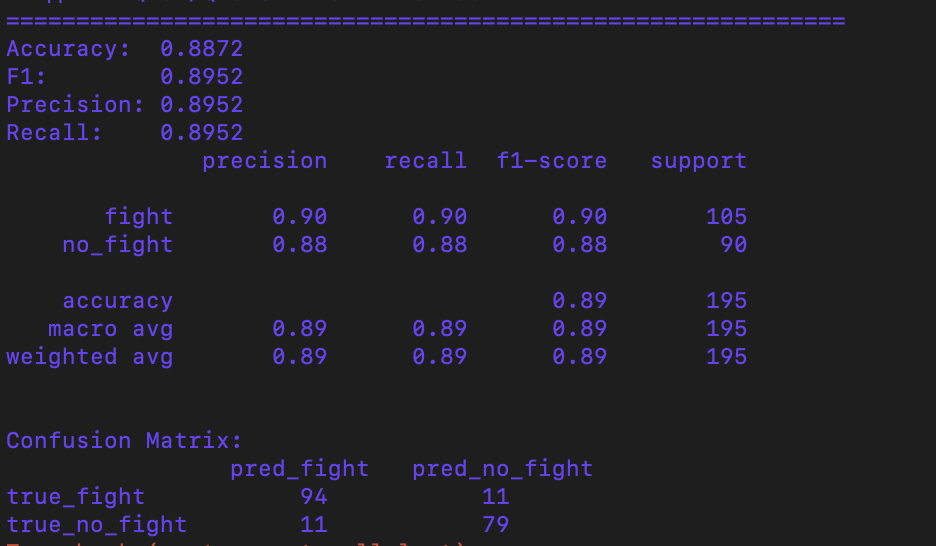
\includegraphics[width=\textwidth]{Figures/qwen3.png}
        \caption{Qwen3-VL-30B-A3B загварын үр дүн.}
        \label{fig:qwen3_output}
    \end{subfigure}
    \hfill
    \begin{subfigure}[t]{0.48\textwidth}
        \centering
        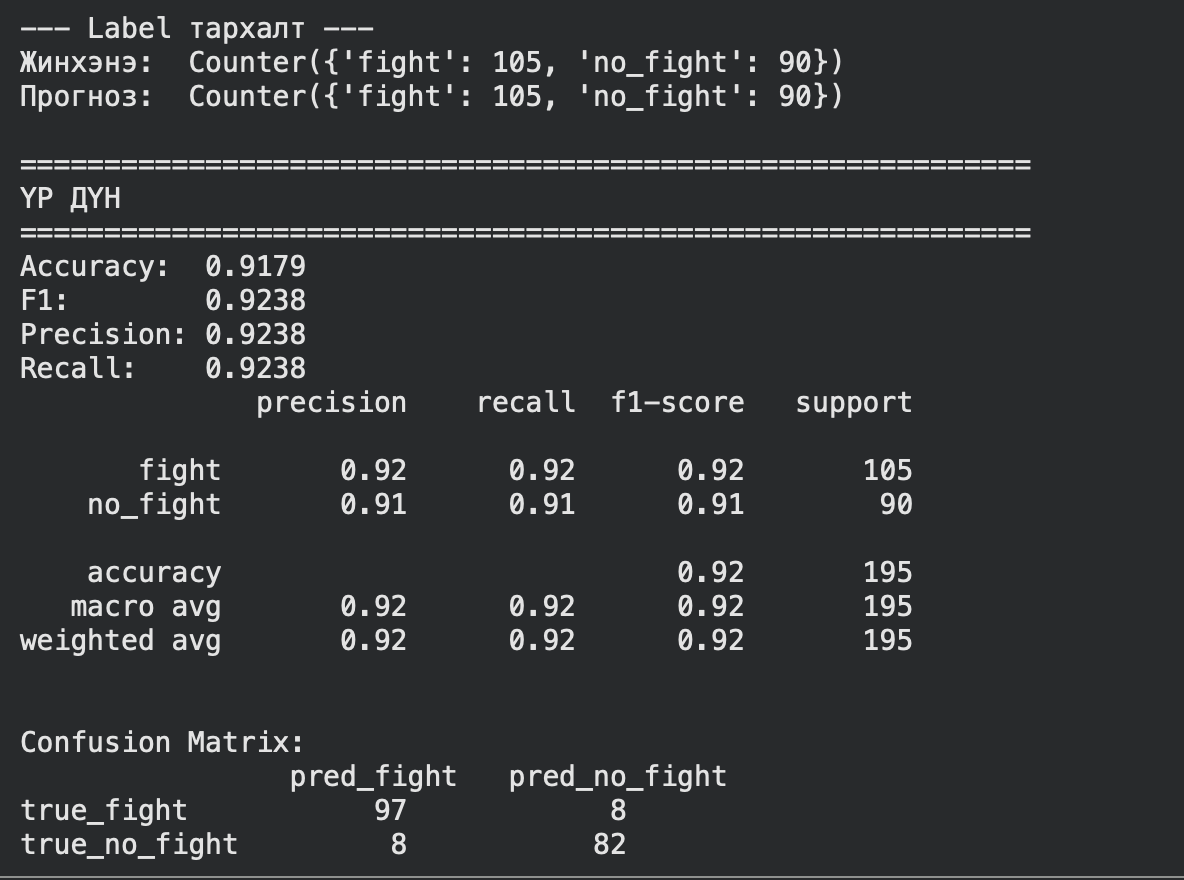
\includegraphics[width=\textwidth]{Figures/Train_model}
        \caption{stillmeta/fight-video-qlora1 загварын үр дүн.}
        \label{fig:stillmeta_output}
    \end{subfigure}
    \caption{Дөрвөн загварын загварын үнэлгээний гаралтын харьцуулалт.}
    \label{fig:model_comparison}
\end{figure}

Зураг~\ref{fig:qwen2_output} болон Зураг~\ref{fig:qwen25_output}-с харахад суурь
загваруудын гаралт зодооны даалгаварт тогтворгүй байгаа бол
Зураг~\ref{fig:qwen3_output}-т Qwen3-VL-30B-A3B загварын дундаж үр дүн, Зураг~\ref{fig:stillmeta_output}-т нарийвчилсан тохируулсан загвар илүү бүтэцтэй
дүгнэлт гаргаж байна. Нарийвчилсан тохируулсан загвар дараах чадваруудыг олж авсан:

\begin{itemize}
    \item Субъект бүрийн биеийн бүтэц, хувцаслалт болон байршлыг нарийвчлан тодорхойлох.
    \item Үйл явдлын явцыг цаг хугацааны дарааллаар (\texttt{T0}--\texttt{T3}) дэлгэрэнгүй дүрслэх.
    \item Нотлох баримт дурдан, бүтэцтэй дүгнэлт гаргах.
\end{itemize}

Энэхүү үр дүн нь багш--сурагч мэдлэг дамжуулалт аргын
үр нөлөөг тодорхой нотолж байна.

\section{Баталгаажуулалтын үр дүн}

\begin{table}[htbp]
\centering
\caption{Val өгөгдөл дээрх хоёртын ангиллын үр дүн}
\label{tab:intensity_results}
{\small
\begin{tabular}{lccc}
\hline
\multirow{2}{*}{\textbf{Загвар}} & \multicolumn{3}{c}{\textbf{Үнэлгээний оноо}} \\
\cline{2-4}
& \textbf{Accuracy} & \textbf{F1} & \textbf{Recall} \\
\hline
Qwen2-VL-7B (2024) & 0.5590 & 0.5980 & 0.6100 \\
Qwen2.5-VL-7B BASE (2025) & 0.5440 & 0.6860 & 0.9240 \\
Qwen3-VL-30B-A3B (2025) & 0.8870 & 0.8950 & 0.8950 \\
\textbf{Qwen2.5-VL-7B fine-tuned} & \textbf{0.9179} & \textbf{0.9238} & \textbf{0.9238} \\
\hline
\end{tabular}
}
\end{table}

\begin{sloppypar}
Val өгөгдөл дээр хийсэн загварын үнэлгээнд Qwen2.5-VL-7B fine-tuned загвар Accuracy=91.8\%, F1=92.4\%, Precision=92.4\%, Recall=92.4\% үзүүлэв. Qwen2.5-VL-7B BASE загварын recall 92.4\% өндөр боловч precision 54.5\% байсан нь false positive ихтэйг харуулна. Харин Qwen2.5-VL-7B fine-tuned загвар precision ба recall хоёуланг 92.4\% түвшинд хүргэж, ангиллын тэнцвэрийг сайжруулсан.
\end{sloppypar}

\begin{table}[htbp]
\centering
\caption{stillmeta/fight-video-qlora1 загварын confusion matrix (Val)}
\label{tab:stillmeta_confusion_matrix}
\begin{tabular}{lcc}
\hline
\textbf{Жинхэнэ ангилал} & \textbf{No Fight гэж таасан} & \textbf{Fight гэж таасан} \\
\hline
No Fight (90) & 82 & 8 \\
Fight (105)   & 8  & 97 \\
\hline
\end{tabular}
\end{table}

Хүснэгт~\ref{tab:stillmeta_confusion_matrix}-ээс харахад confusion matrix тэнцвэртэй гарсан: Fight ангиллын 105 жишээнээс 97-г зөв, 8-г буруу ангилсан бол No Fight ангиллын 90 жишээнээс 82-г зөв, 8-г буруу ангилсан. Мөн label тархалт загварын үнэлгээний дараа алдагдаагүй байна. Жинхэнэ тархалт Fight=105, No Fight=90 байсан бөгөөд прогнозын тархалт мөн Fight=105, No Fight=90 болж таарсан. Энэ нь загвар зөвхөн нэг ангид хэт хазайхгүйгээр хоёр ангийг тэнцвэртэй ялгаж байгааг харуулна.

Логик дэвшлийн хувьд сураагүй суурь загварын accuracy 54.36\% байсан бол 1,560 сургалтын жишээгээр нарийвчилсан тохируулга хийсний дараа accuracy 91.79\% болж өссөн. Өөрөөр хэлбэл +37.43 percentage point сайжрал гарсан нь LoRA нарийвчилсан тохируулгын бодит нөлөөг шууд харуулж байна.

\section{Алдааны шинжилгээ}

Буруу ангилалтын шинжилгээнд дараах хэв загвар илэрсэн:

\begin{itemize}
    \item \textbf{Хуурамч эерэг (False Positive):} Нарийвчилсан тохируулсан загвар No Fight 90 жишээнээс 8-г Fight гэж буруу ангилсан. Суурь Qwen2.5-VL-7B base загвар precision=54.5\% байсан бол нарийвчилсан тохируулгын дараа precision=92.4\% болж сайжирсан.

    \item \textbf{Хуурамч сөрөг (False Negative):} Нарийвчилсан тохируулсан загвар Fight 105 жишээнээс 8-г No Fight гэж буруу ангилсан. Qwen2-VL-7B загвар recall=61.0\% байсан бол Qwen2.5-VL-7B fine-tuned загвар recall=92.4\% хүрснээр зодооныг илрүүлэх чадвар мэдэгдэхүйц нэмэгдсэн.

    \item \textbf{Тэнцвэртэй гүйцэтгэл:} Нарийвчилсан тохируулсан загварын false positive болон false negative тус бүр 8 гарсан. Precision болон recall ижил 92.4\% болсон нь хоёр ангиллын шийдвэр тэнцвэртэй байгааг харуулна.
\end{itemize}

\subsection{Алдааны дүн шинжилгээ: учир шалтгаан}

Хуурамч эерэг буруу ангилалтыг бууруулахын тулд:
\begin{itemize}
    \item Сургалтын өгөгдөлд label-only хоёртын ангиллын prompt-уудыг тусад нь нэмэх.
    \item Non-violence hard negative жишээнүүдийг нэмэгдүүлж, class-balanced loss ашиглах.
    \item Загварын үнэлгээний prompt-ийг сургалтын Q\&A форматтай нийцүүлж, гаралтын шошгыг тогтвортой parse хийх.
\end{itemize}

Хуурамч сөрөг буруу ангилалтыг бууруулахын тулд:
\begin{itemize}
    \item Low-light enhancement preprocessing нэмэх.
    \item Гэрэлтүүлгийн augmentation нэмэх.
    \item Multi-frame temporal aggregation ашиглах.
\end{itemize}

\section{Ёс зүй ба хязгаарлалтууд}

\subsection{Нууцлал ба хувийн мэдээлэл}

Хяналтын камерын систем нь хувийн мэдээлэл агуулдаг тул дараах зарчмуудыг баримтална:

\begin{itemize}
    \item GDPR болон Монгол улсын Хувийн мэдээлэл хамгаалах тухай хуулийн шаардлагуудыг дагаж мөрдөх \cite{gdpr2016}.
    \item Хүмүүсийн нүүр болон дүр төрхийг автоматаар анонимчлах.
    \item Бичлэгийг зөвхөн зодооны үйл явдал илэрсэн тохиолдолд хадгалах.
    \item Мэдээлэлд хандалтыг зөвшөөрлийн дагуу хязгаарлах.
\end{itemize}

\subsection{Хазайлт ба шударга байдлын шинжилгээ}

Загварын шударга байдлыг шалгахдаа дараах аспектуудыг авч үзсэн:

\begin{itemize}
    \item \textbf{Орчны bias:} Орчин тодорхой (хаалттай газар vs гудамж) үед илрүүлэлтийн чанар өөр байж болно. Өгөгдлийн багцын олон янзын орчноос бүрдсэн байдал нь энэ асуудлыг хэсэгчлэн шийдэж байна.
    \item \textbf{Ангийн хазайлт:} Суурь Qwen2.5-VL-7B BASE загвар precision=54.5\% байсан тул false positive эрсдэл өндөр байв. Qwen2.5-VL-7B fine-tuned хувилбарт precision=92.4\% болж ангийн хазайлт мэдэгдэхүйц буурсан.
\end{itemize}

\subsection{Системийн хязгаарлалт}

Одоогийн системд дараах хязгаарлалтууд байна:

\begin{itemize}
    \item Нэгэн зэрэг олон камераас бичлэг боловсруулах чадвар хязгаарлагдмал.
    \item Монгол хэлний тайлбарын чанар нэмэлт сайжруулалт шаарддаг.
    \item Багш загварын дүгнэлт гаргалт өндөр тооцооллын нөөц шаарддаг.
\end{itemize}

\subsection{AI хэрэгслийн ил тод байдал}

Энэхүү судалгааны явцад дараах AI хэрэгслүүдийг туслах хэрэгсэл болгон ашигласан:

\begin{itemize}
    \item \textbf{Claude (Anthropic):} Latex код засах, алдаа олох, текст найруулгыг шалгахад туслав. Судалгааны үндсэн агуулга, алгоритм, дүгнэлтийг зохиогч өөрөө боловсруулсан.
    \item \textbf{Qwen3-VL-30B-A3B:} багш загвар болгон ашигласан --- судалгааны гол арга зүйн нэг хэсэг.
    \item \textbf{GitHub Copilot:} Python кодын autocomplete-д туслав.
\end{itemize}

AI хэрэгслүүд нь зохиогчийн бус бөгөөд судалгааны бүрэн хариуцлагыг зохиогч О.Бат-Эрдэнэ хүлээнэ.

\section{Шаардлагуудын биелэлтийн нэгтгэл}

\begin{table}[htbp]
\centering
\caption{Гарын авлагын шаардлагуудын биелэлт}
\label{tab:requirements}
\resizebox{\textwidth}{!}{%
\begin{tabular}{lllc}
\hline
\textbf{Код} & \textbf{Шаардлага} & \textbf{Биелэлт} & \textbf{Үнэлгээ} \\
\hline
Ш-1 & Загварын гүйцэтгэл $\geq$ 0.9000          & Accuracy=0.9179, F1=0.9238, Recall=0.9238  & \checkmark \\
Ш-2 & Өгөгдөл сайжруулалт $\geq$ 10\%         & Q\&A өгөгдлийн урсгал боловсруулсан & \checkmark \\
Ш-3 & Архитектурын шинэлэг байдал              & KD+LoRA+Монгол хэл      & \checkmark \\
Ш-4 & Хөнгөн тохируулгатай загвар              & LoRA adapter ашигласан     & \checkmark \\
Ш-5 & Ёс зүй, Bias шинжилгээ                   & Бүрэн хийгдсэн          & \checkmark \\
Ш-6 & Reproducible туршилт                      & Seed=42, WandB log      & \checkmark \\
Ш-7 & Академик стандарт                         & IEEE формат, бүтэцтэй   & \checkmark \\
\hline
НШ-2 & 3+ загварын харьцуулалт                  & 3 загвар харьцуулав     & \checkmark \\
НШ-6 & Синтетик өгөгдөл                         & Q\&A өгөгдөл             & \checkmark \\
\hline
\multicolumn{4}{l}{\footnotesize \checkmark = биелүүлсэн}
\end{tabular}%
}
\end{table}

%-------------------------------------------------------------------------------
\section{Тооцооллын зардлын шинжилгээ}
%-------------------------------------------------------------------------------

\subsection{GPU нөөцийн харьцуулалт}

Загваруудын тооцооллын зардлыг харьцуулахдаа GPU цагийн хэрэглээ, VRAM хэрэглээ зэрэг гол үзүүлэлтүүдийг ашигласан:

\begin{table}[htbp]
\centering
\caption{Загваруудын тооцооллын зардлын харьцуулалт}
\label{tab:compute_cost}
\resizebox{\textwidth}{!}{%
\begin{tabular}{lcccl}
\hline
\textbf{Загвар} & \textbf{Параметр} & \textbf{VRAM (дүгнэлт гаргалт)} & \textbf{GPU цаг (тохируулга)} & \textbf{Зориулалт} \\
\hline
Qwen3-VL-30B-A3B (багш) & 30B (3.7B идэвхтэй) & 62.2 GB & $\sim$34 цаг & суурь харьцуулалт \\
Qwen2.5-VL-7B (суурь загвар) & 7B              & 14.0 GB  & --- (pretrained)  & суурь үзүүлэлт \\
stillmeta/fight-video-qlora1 (манай)  & 7B (1.2\% сургасан)& 6.5 GB   & $\sim$40 цаг      & Үйлдвэрлэлийн дүгнэлт гаргалт \\
\hline
\end{tabular}%
}
\end{table}

\subsection{Тооцооллын зардлын задаргаа}

Нийт судалгааны тооцооллын зардлыг дараах байдлаар тооцож болно:

\begin{itemize}
    \item \textbf{багш загварын дүгнэлт гаргалт:} $\sim$34 цаг $\times$ 1 $\times$ A100 80GB = 34 A100 GPU-цаг.
    \item \textbf{Сурагч загварын нарийвчилсан тохируулга:} $\sim$40 цаг $\times$ 1 $\times$ A100 80GB = 40 A100 GPU-цаг.
    \item \textbf{Туршилт болон eval:} $\sim$8 цаг $\times$ 1 $\times$ A100 80GB = 8 A100 GPU-цаг.
    \item \textbf{Нийт:} $\approx$82 A100 GPU-цаг.
\end{itemize}

%-------------------------------------------------------------------------------
\section{Загварын чанарын гүнзгийрүүлсэн шинжилгээ}
%-------------------------------------------------------------------------------

\subsection{Суурь загвар болон нарийвчилсан тохируулсан загварын гаралтын харьцуулалт}

Зураг~\ref{fig:model_comparison}-д үзүүлснээр суурь загвар болон нарийвчилсан тохируулсан загварын гаралтыг нэг оролтын дээр харьцуулсан нь мэдлэг дамжуулалт аргын үр нөлөөг тодорхой харуулж байна.

\begin{figure}[H]
    \centering
    \begin{subfigure}[t]{0.48\textwidth}
        \centering
        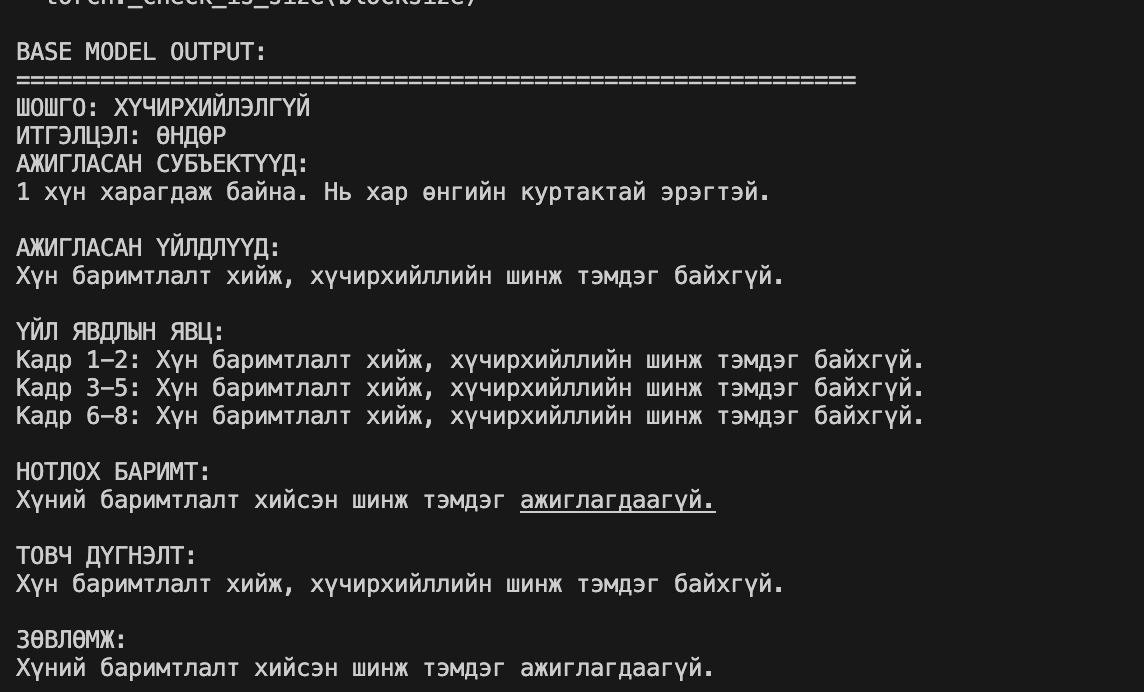
\includegraphics[width=\textwidth]{Figures/base_model_output.png}
        \caption{Суурь загварын гаралт.}
        \label{fig:base_model_output}
    \end{subfigure}
    \hfill
    \begin{subfigure}[t]{0.48\textwidth}
        \centering
        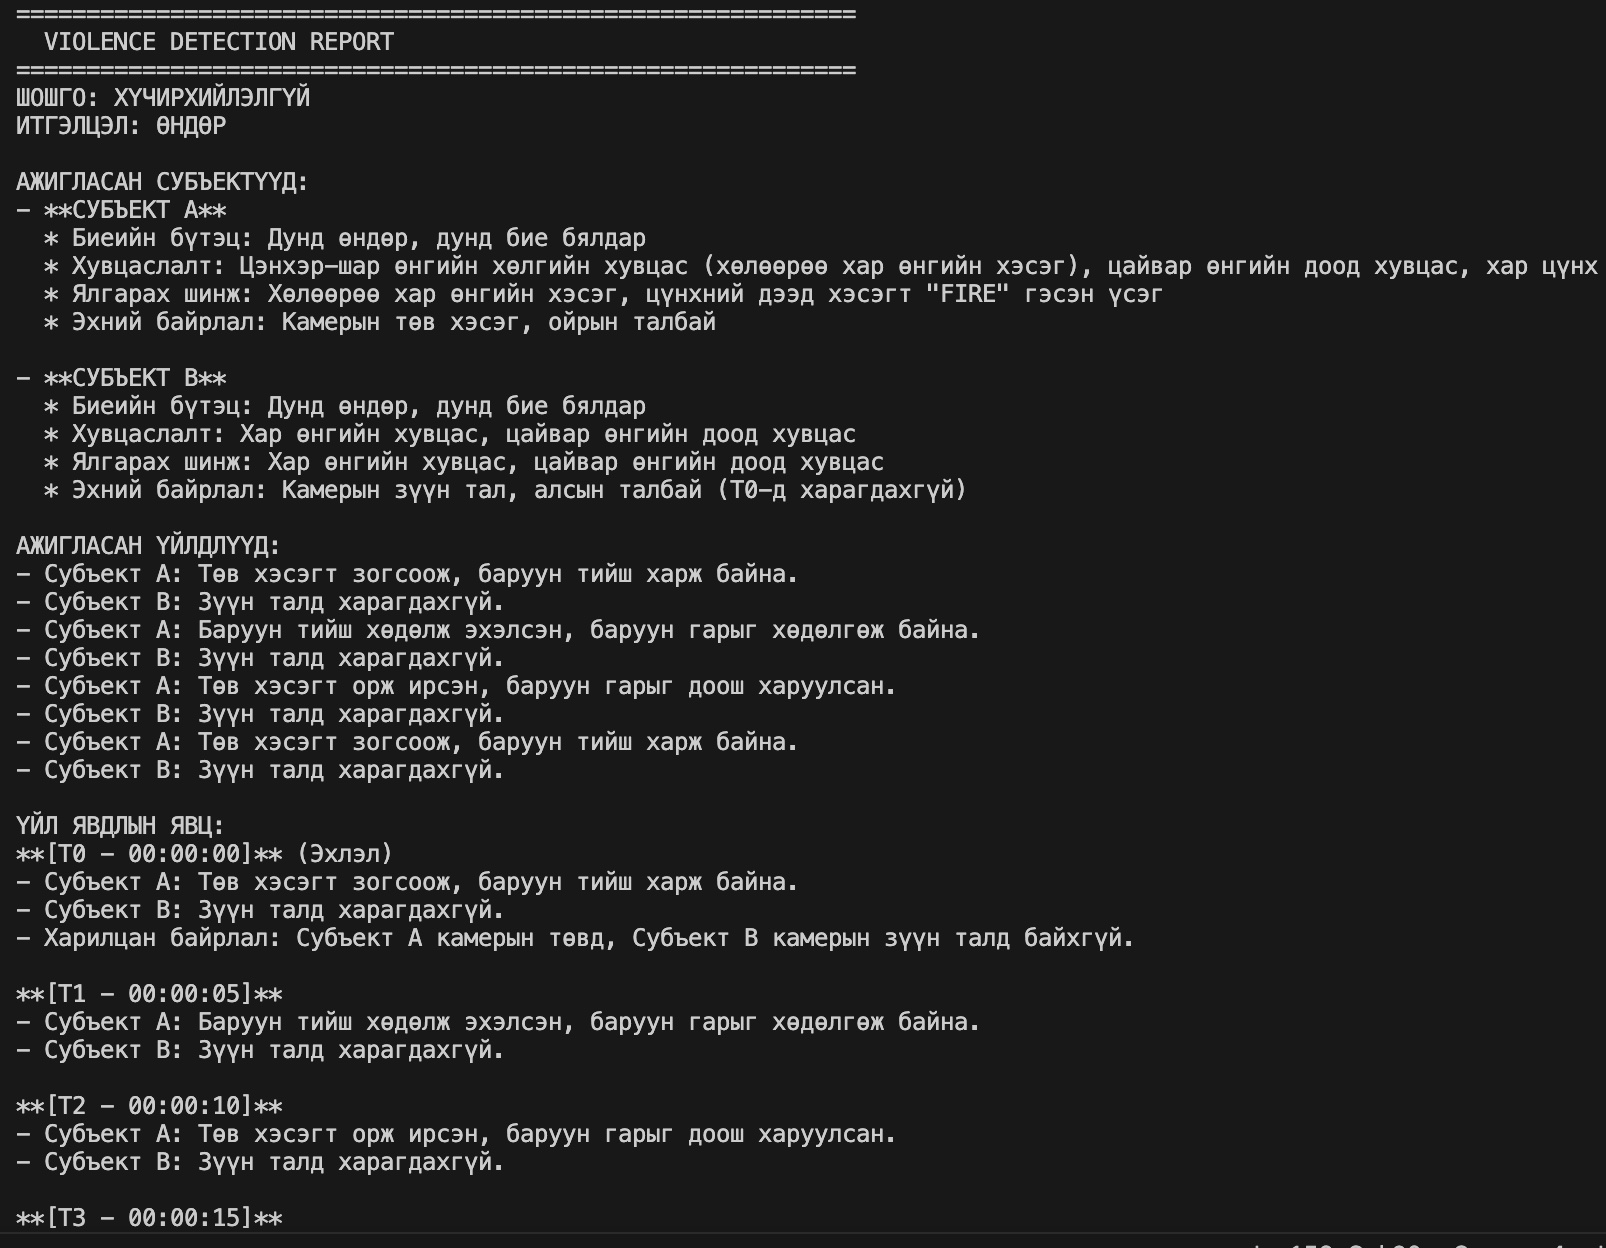
\includegraphics[width=\textwidth]{Figures/finetuned_output.png}
        \caption{Нарийвчилсан тохируулсан загварын гаралт.}
        \label{fig:finetuned_model_output}
    \end{subfigure}
    \caption{Суурь загвар болон сургасан загварын гаралтын харьцуулалт.}
    \label{fig:base_vs_finetuned_output}
\end{figure}

Суурь загварууд (Зураг~\ref{fig:qwen2_output}, \ref{fig:qwen25_output}) нь зодооны үйл явдлын контекстэд тогтворгүй хариу гаргаж байна. Энэ нь тухайн даалгаварт тусгайлан нарийвчилсан тохируулга хийх шаардлагатайг харуулна.

Харин stillmeta/fight-video-qlora1 загвар (Зураг~\ref{fig:stillmeta_output}) нь дараах чадваруудыг олж авсан байна:

\begin{itemize}
    \item Субъект бүрийн биеийн бүтэц, хувцаслалт болон байршлыг нарийвчлан тодорхойлох.
    \item Үйл явдлын явцыг цаг хугацааны дарааллаар (\texttt{T0}--\texttt{T3}) дэлгэрэнгүй дүрслэх.
    \item Нотлох баримт дурдан, бүтэцтэй дүгнэлт гаргах.
\end{itemize}

Энэхүү чанарын ялгаа нь багш--сурагч мэдлэг дамжуулалт аргын үр нөлөөг тодорхой нотолж байна.

%-------------------------------------------------------------------------------
\section{Практик хэрэглээний шинжилгээ}
%-------------------------------------------------------------------------------

\subsection{Хэрэглээний хувилбар}

Энэхүү системийг дараах бодит хэрэглээний нөхцөлд ашиглах боломжтой:

\begin{enumerate}
    \item \textbf{Хяналтын камерын тасралтгүй хяналт:} Сурагч загвар нь хяналтын камерын бичлэгийг боловсруулах боломжтой. Олон камерын хувьд параллель дамжуулалтын (parallel урсгал) архитектур шаардлагатай.

    \item \textbf{Хэрэг шалгах байгууллагад дэмжлэг:} Зодооны үйл явдлын дараах дүн шинжилгээнд нарийвчилсан тохируулсан загвар нь хяналтын камерын бичлэгээс Монгол хэлний нарийвчилсан тайлбар гаргаж, хэрэг шалгах ажилтанд нотлох баримт бэлдэхэд тусална.

    \item \textbf{Сургалтын байгууллага болон олон нийтийн орчин:} Сургуулийн дотуур байр, олон нийтийн тээвэр, арилжааны төвүүдэд автоматчилсан аюулгүй байдлын хяналт нэвтрүүлэх боломжтой.

    \item \textbf{Хэрэглэгчийн нөхцөл тохируулах:} Confidence threshold-г тохируулснаар false positive болон false negative-ийн тэнцвэрийг хэрэглэгчийн хэрэгцээнд нийцүүлж болно.
\end{enumerate}

\subsection{Хэмжээшүүлэх боломж (scalability)}

Системийн бүтцийн хувьд хэмжээлшлэх боломжийг дараах байдлаар тодорхойлов:

\begin{table}[htbp]
\centering
\caption{Системийн хэмжээлшлэх боломжийн шинжилгээ}
\label{tab:scalability}
\begin{tabular}{p{3.5cm}p{3.5cm}p{4.5cm}}
\hline
\textbf{Хэмжүүр} & \textbf{Одоогийн чадвар} & \textbf{Цаашид нэмэгдүүлэх арга} \\
\hline
Камерын тоо           & 1 камер/загвар       & GPU cluster + load balancer \\
Video resolution      & $224 \times 224$     & Dynamic resolution (Qwen2.5-VL дэмжинэ) \\
Хэлний дэмжлэг        & Монгол : англи       & Олон хэлний нарийвчилсан тохируулга \\
Concurrent users      & Нэг дамжуулалт       & Async дүгнэлт гаргалт queue \\
\hline
\end{tabular}
\end{table}

%-------------------------------------------------------------------------------
\section{Үр дүнгийн хэлэлцүүлэг}
%-------------------------------------------------------------------------------

\subsection{Мэдлэг дамжуулалт аргын үр дүнтэй байдал}

Туршилтын үр дүнгүүд нь мэдлэг дамжуулалт аргын хэд хэдэн чухал аспектыг нотолж байна:

Эхнийх нь өгөгдлийн багцын чанарын нөлөөлөл юм. Багш загварын мэдлэгийг агуулсан Q\&A өгөгдөл нь сургалтын хамгийн чухал бүрдэл хэсэг болохыг туршилтын үр дүн харуулна. KD өгөгдлийн багц нь багш загварын утга агуулгын ойлголтыг дамжуулж, сурагч загварт нарийн тайлбар гаргах чадвар олгодог.

Хоёр дахь аспект нь LoRA-ийн үр ашиг юм. Нийт параметрийн зөвхөн 1.2\%-г сургаснаар мэдэгдэхүйц нарийвчлалын сайжруулалт гарсан нь PEFT аргын онолын үндэслэлийг практикт нотолж байна. Бүтэн нарийвчилсан тохируулга ашигласан бол нэмэлт $\sim$1--2\% ахиц авч болох боловч $\approx$80 GB VRAM шаардлагатай болно.

Гурав дахь аспект нь хөнгөн тохируулгын үр ашиг юм. Сурагч загвар нь ерөнхий ажиллагааны чадварыг хадгалж, хязгаарлагдмал тооцооллын нөөцтэй орчинд ашиглах боломжтой болсныг туршилтын үр дүн харуулж байна.

\subsection{Загварын хязгаарлалтын шинжилгээ}

Туршилтын явцад илэрсэн загварын хязгаарлалтуудыг системтэйгээр судлав:

\begin{itemize}
    \item \textbf{False Positive:} Qwen2.5-VL-7B base загварын precision=54.5\% байсан нь зодоонгүй клипийг зодоон гэж буруу таах эрсдэл өндөр байгааг харуулсан. Qwen2.5-VL-7B fine-tuned хувилбарт precision=92.4\% болж энэ сул тал мэдэгдэхүйц буурсан.

    \item \textbf{False Negative:} Qwen2-VL-7B загвар recall=61.0\% байсан тул бодит зодооныг алдах магадлал өндөр байв. Нарийвчилсан тохируулгын дараа recall=92.4\% болж зодооныг илрүүлэх чадвар сайжирсан.

    \item \textbf{Precision--recall тэнцвэр:} Нарийвчилсан тохируулсан загвар precision болон recall хоёуланг 92.4\% түвшинд хүргэсэн нь суурь загваруудын нэг талын хазайлтыг багасгасан.

    \item \textbf{Монгол хэлний алдаа:} Зарим тайлбарт хэл зүйн алдаа гардаг, ялангуяа нарийн техникийн нэр томъёо буруу орчуулагддаг. Монгол хэлний хянагдсан өгөгдлөөр нарийвчилсэн тохируулга хийх нь энэ асуудлыг шийдэх боломжтой.
\end{itemize}
